%%%%%%%%%%%%%%%%%%%%%%%%%%%%%%%%%%%%%%%%%
% Beamer Presentation
% LaTeX Template
% Version 1.0 (10/11/12)
%
% This template has been downloaded from:
% http://www.LaTeXTemplates.com
%
% License:
% CC BY-NC-SA 3.0 (http://creativecommons.org/licenses/by-nc-sa/3.0/)
%
%%%%%%%%%%%%%%%%%%%%%%%%%%%%%%%%%%%%%%%%%

%----------------------------------------------------------------------------------------
%	PACKAGES AND THEMES
%----------------------------------------------------------------------------------------

\documentclass{beamer}

\mode<presentation> {

% The Beamer class comes with a number of default slide themes
% which change the colors and layouts of slides. Below this is a list
% of all the themes, uncomment each in turn to see what they look like.

%\usetheme{default}
%\usetheme{AnnArbor}
%\usetheme{Antibes}
%\usetheme{Bergen}
%\usetheme{Berkeley}
%\usetheme{Berlin}
%\usetheme{Boadilla}
%\usetheme{CambridgeUS}
%\usetheme{Copenhagen}
%\usetheme{Darmstadt}
%\usetheme{Dresden}
%\usetheme{Frankfurt}
%\usetheme{Goettingen}
%\usetheme{Hannover}
%\usetheme{Ilmenau}
%\usetheme{JuanLesPins}
%\usetheme{Luebeck}
\usetheme{Madrid}
%\usetheme{Malmoe}
%\usetheme{Marburg}
%\usetheme{Montpellier}
%\usetheme{PaloAlto}
%\usetheme{Pittsburgh}
%\usetheme{Rochester}
%\usetheme{Singapore}
%\usetheme{Szeged}
%\usetheme{Warsaw}

% As well as themes, the Beamer class has a number of color themes
% for any slide theme. Uncomment each of these in turn to see how it
% changes the colors of your current slide theme.

%\usecolortheme{albatross}
%\usecolortheme{beaver}
%\usecolortheme{beetle}
%\usecolortheme{crane}
%\usecolortheme{dolphin}
%\usecolortheme{dove}
%\usecolortheme{fly}
%\usecolortheme{lily}
%\usecolortheme{orchid}
%\usecolortheme{rose}
%\usecolortheme{seagull}
%\usecolortheme{seahorse}
%\usecolortheme{whale}
%\usecolortheme{wolverine}

%\setbeamertemplate{footline} % To remove the footer line in all slides uncomment this line
%\setbeamertemplate{footline}[page number] % To replace the footer line in all slides with a simple slide count uncomment this line

\setbeamertemplate{navigation symbols}{} % To remove the navigation symbols from the bottom of all slides uncomment this line
}

\usepackage{graphicx} % Allows including images
\usepackage{booktabs} % Allows the use of \toprule, \midrule and \bottomrule in tables
\usepackage[utf8]{inputenc}
\usepackage[T1]{fontenc}

\usepackage{hyperref}
\definecolor{links}{HTML}{3578cc}
\hypersetup{colorlinks,linkcolor=,urlcolor=links}

%----------------------------------------------------------------------------------------
%	TITLE PAGE
%----------------------------------------------------------------------------------------

\title[Protein Graph DB]{ Protein Graph Database } % The short title appears at the bottom of every slide, the full title is only on the title page

\author{ Borna Bešić, Dilmurat Yusuf } % Your name
\institute[] % Your institution as it will appear on the bottom of every slide, may be shorthand to save space
{
Bioinformatics Group \\
\medskip
Albert-Ludwigs-Universität, Freiburg  % Your institution for the title page
}
\date{\today} % Date, can be changed to a custom date

\begin{document}

\begin{frame}
\titlepage % Print the title page as the first slide
\end{frame}

%----------------------------------------------------------------------------------------
%	PRESENTATION SLIDES
%----------------------------------------------------------------------------------------

\AtBeginSection[]{
    \begin{frame}{Overview}
        \tableofcontents[currentsection, hideothersubsections]
    \end{frame}
}

%------------------------------------------------
\section{Introduction} % Sections can be created in order to organize your presentation into discrete blocks, all sections and subsections are automatically printed in the table of contents as an overview of the talk
%------------------------------------------------

\begin{frame}{Protein network}
\begin{figure}
    \centering
    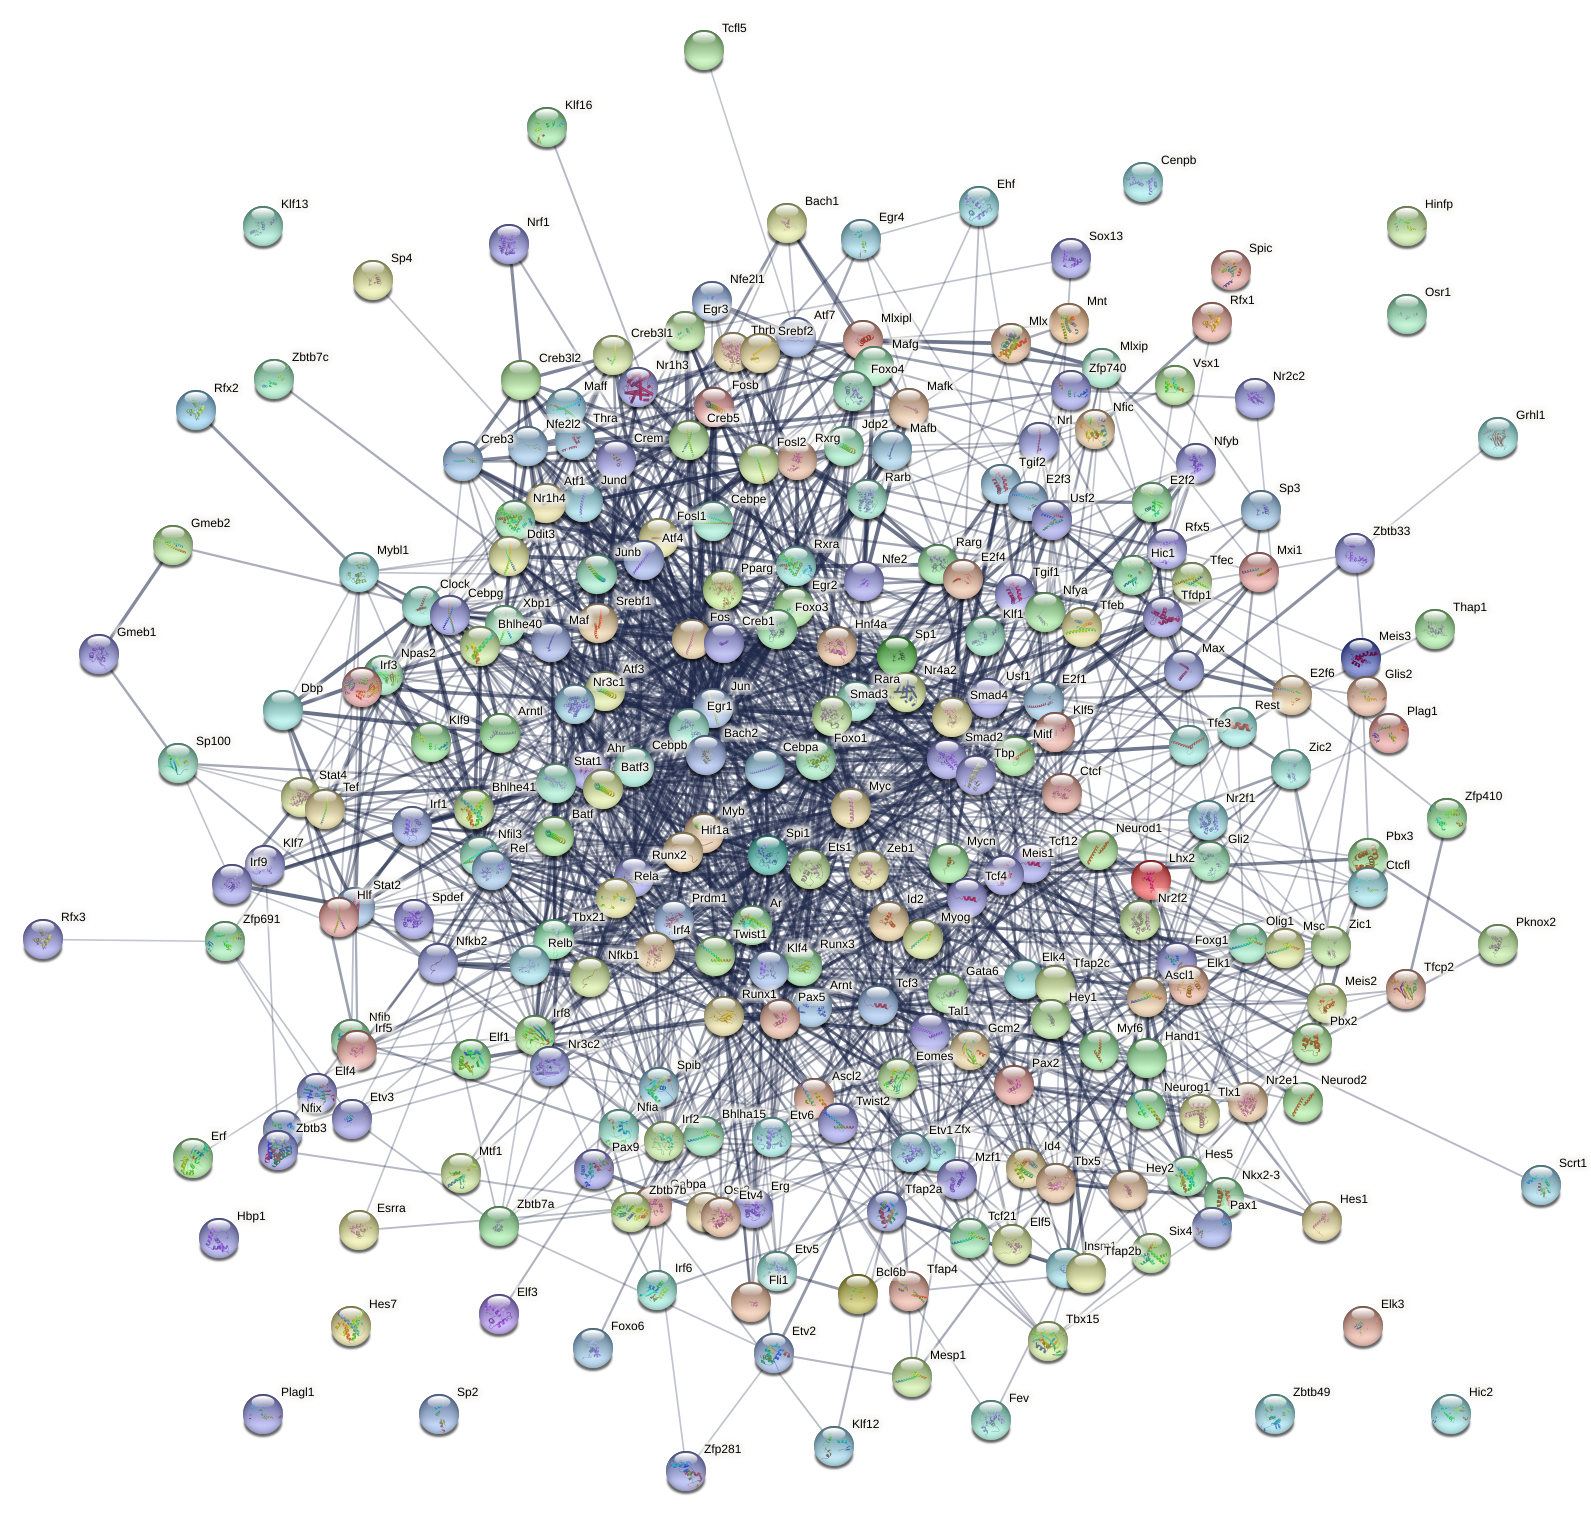
\includegraphics[width=0.55\linewidth]{protein_network_example.png}
\end{figure}

\end{frame}
%------------------------------------------------



\begin{frame}{Neo4j graph database}
% NOTE:
% e, com and cty are variables used to represent the nodes
% If a reference to a node is not needed, variable name can be left out
% All of this could have been created in a single CREATE statement, but is more
% readable like this
% CREATE statement must contain directed relationships
    \begin{block}{Cypher}
        % \scriptsize
        % CREATE (e:Employee \{ name: "Amy Peters", date\_of\_birth: "1984-03-01", employee\_ID: 1\})\newline
        % CREATE (com:Company)\newline
        % CREATE (cty:City)\newline
        % CREATE (com)-[:HAS\_CEO \{start\_date: "2008-01-20"\}]->(e)\newline
        % CREATE (com)-[:LOCATED\_IN]->(cty)
        \begin{figure}
            \centering
            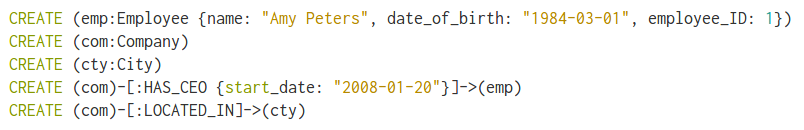
\includegraphics[width=\linewidth]{create_query.png}
        \end{figure}
    \end{block}
    \begin{figure}
        \centering
        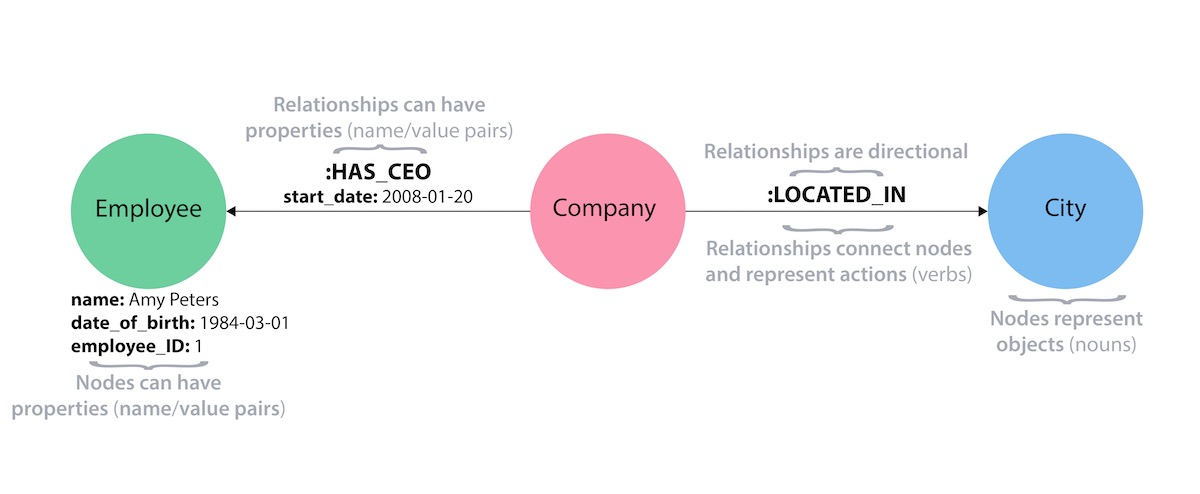
\includegraphics[clip=true,width=\linewidth]{property_graph_elements.jpg}
    \end{figure}
\end{frame}

\begin{frame}{Neo4j graph database}
% NOTE
% Redundancy: SQL has to use duplicate ID columns in tables that have to be joined
% Design change: Change in one SQL table usually requires other tables to change

% \begin{block}{Example of a Cypher query}
% MATCH (:person \{ name: "Alan" \})-[p:PURCHASED]-\textgreater(b:book) \\
% RETURN p.date, b
% \end{block}
\begin{itemize}
    \item Pros:
    \begin{itemize}
        \item Outperforming RDBMS for associative data
        \item No redundancy %Q: in what context?
        \item Easier to implement a design change
    \end{itemize}
    \vfill
    \item Cons:
    \begin{itemize}
        \item Not standard; new query language (Cypher)
        \item Harder to do summing queries and max queries efficiently %NOTE: https://medium.com/@mtbuzzerseo/graph-database-vs-relational-database-e5798281f6ef
    \end{itemize}
\end{itemize}
\end{frame}

\begin{frame}{Neo4j graph database}
Intuitive and concise query
% NOTE:
% START statement in the Cypher query was used in Neo4j 1.x and may be deprecated soon.
% From Neo4j 2.0, only MATCH wirh WHERE is preferred.

% NOTE:
% Neo4j is a graph database but still returns results in the table form
    \begin{figure}
        \centering
        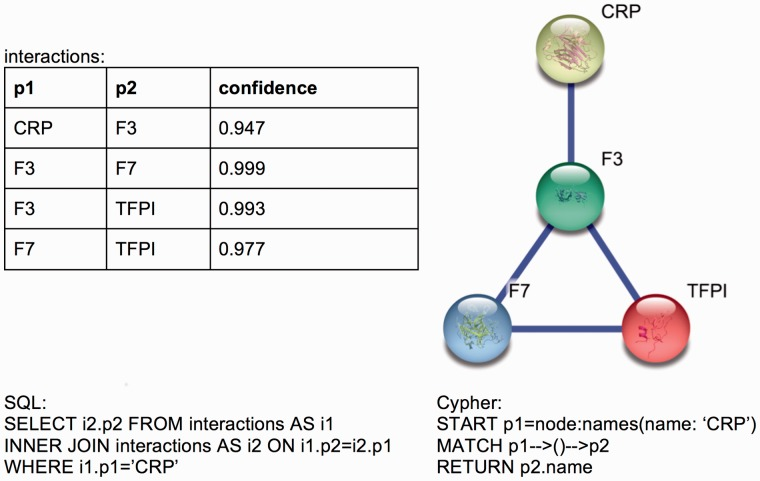
\includegraphics[width=0.7\linewidth]{relational_vs_graph.jpg}
        \caption{\href{https://www.ncbi.nlm.nih.gov/pmc/articles/PMC3842757/}{Have CT, Jensen LJ. Are graph databases ready for bioinformatics?}}
    \end{figure}
\end{frame}

\begin{frame}{Neo4j graph database}
Speed
    \begin{figure}
        \centering
        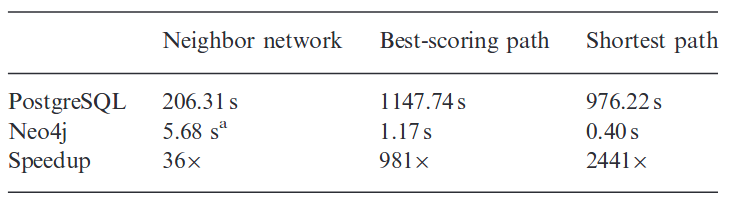
\includegraphics[width=0.7\linewidth]{graph-dbs-benchmark.png}
        \caption{\href{https://www.ncbi.nlm.nih.gov/pmc/articles/PMC3842757/}{Have CT, Jensen LJ. Are graph databases ready for bioinformatics?}}
    \end{figure}
\end{frame}

\begin{frame}{What do we want?}

\begin{itemize}
    \item A graph database of protein association
    \begin{itemize}
        \item Intutive graph model 
        \item Queries: concise, intuitive and efficient
        \item Dynamic web user interface % NOTE: We are not in 1990s, everything in one page, no refreshing
    \end{itemize}
    \vfill
    \item Integration of different types of information
    \begin{itemize}
        \item Protein association
        \item Pathway, class
        \item Disease, drug, compound
    \end{itemize}
    \vfill
\end{itemize}
\end{frame}

% \begin{frame}
% \frametitle{Cytokines}
% \begin{itemize}
%     \item Molecular messengers between cells
%     \item Interact with cells of the immune system
%     \item Regulate the body's response to disease and infection
%     \item Mediate normal cellular processes in the body
% \end{itemize}
% \begin{figure}
%     \centering
%     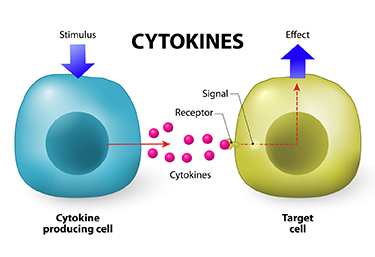
\includegraphics[width=0.5\linewidth]{cytokines.jpg}
% \end{figure}
% \end{frame}

%------------------------------------------------

\section{Methodology}
\begin{frame}{Sources of data}
\begin{columns}[c] % The "c" option specifies centered vertical alignment while the "t" option is used for top vertical alignment

\column{.5\textwidth} % Left column and width
\begin{figure}
    \centering
    
\includegraphics[width=1\linewidth]{string_logo.png}
\end{figure}
\begin{itemize}
    \item \href{https://string-db.org/}{STRING}
    \begin{itemize}
        \item proteins
        \item protein - protein associations
    \end{itemize}
\end{itemize}

\column{.5\textwidth}
\begin{figure}
    \centering
    
\includegraphics[width=0.9\linewidth]{kegg_logo.png}
\end{figure}
\begin{itemize}
    \item \href{https://www.genome.jp/kegg/pathway.html}{KEGG PATHWAY}
    \begin{itemize}
        \item pathways
        \begin{itemize}
            \item classes
            \item compounds
            \item drugs
            \item diseases
        \end{itemize}
    \end{itemize}
\end{itemize}

\end{columns}
\end{frame}

\begin{frame}{STRING}
% NOTE:
% STRING also offers a REST API, which we used for mapping the identifiers
    \begin{itemize}
        \item Database of known and predicted protein-protein interactions
        \vfill
        \item 7 score channels $ \rightarrow $ combined score
        \begin{enumerate}
            \item Experiments
            \item Database
            \item Textmining
            \item Co-expression
            \item Neighbourhood
            \item Fusion
            \item Co-occurence
        \end{enumerate}
        \vfill
        \item One of best in overall performance for recovery of disease gene sets (\href{https://www.ncbi.nlm.nih.gov/pubmed/29605183}{Huang et al., Systematic Evaluation of Molecular Networks for Discovery of Disease Genes, Cell Systems})
        \vfill
        \item Full database dumps available for download: 512.8 GB (compressed)
    \end{itemize}
\end{frame}

\begin{frame}{STRING Schema}
% NOTE:
% Dump cannot be loaded on a local computer because of the size
% Join on different column names (different names for the same thing in different tables)
% STRING documentation is not perfect, but guides you in a right direction (~ 10 tables manually checked)
% Because of the license issues, STRING does not provide KEGG data in their dumps
% 

\begin{figure}
    \centering
    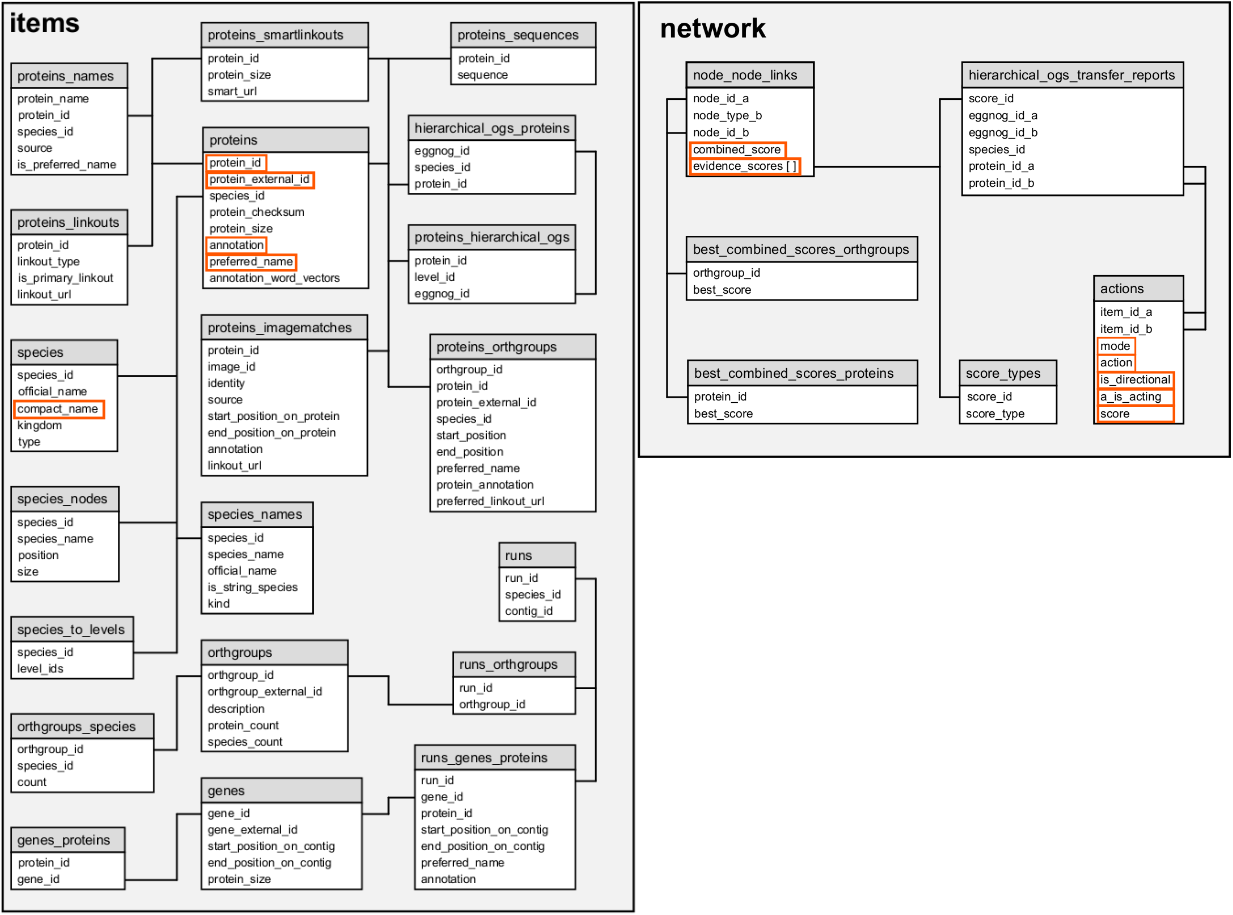
\includegraphics[width=\linewidth]{string-tables.png}
\end{figure}
\end{frame}

\begin{frame}{KEGG PATHWAY Flat file}
% NOTE:
% KEGG uses genes while STRING uses proteins
% Some of the KEGG genes were not able to be mapped to STRING proteins
% Not a defined format; various number of whitespaces in rows
% https://backofenlab.github.io/protein-graph-database/KEGG
\begin{figure}
    \centering
    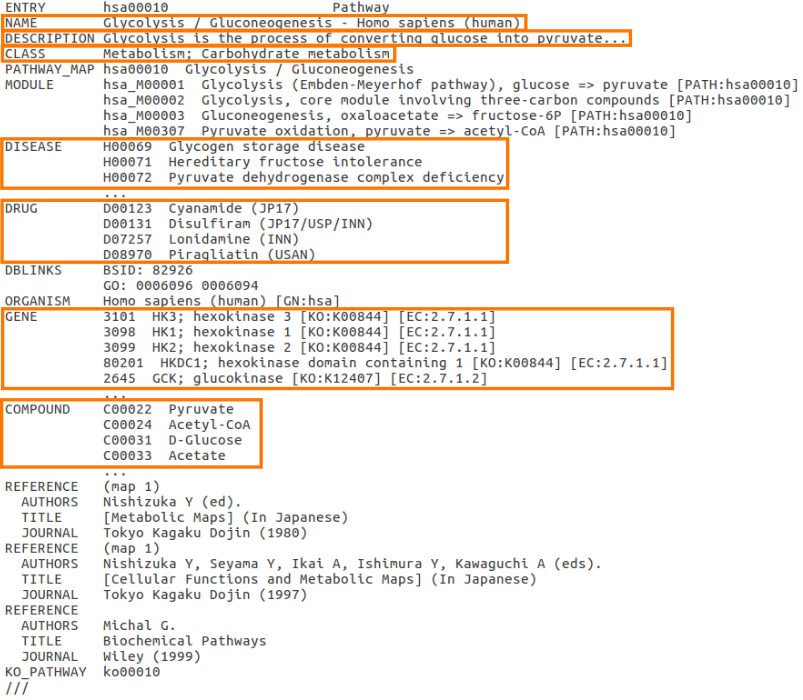
\includegraphics[width=0.8\linewidth]{kegg-flat-file.png}
\end{figure}
\end{frame}

\begin{frame}
\frametitle{Protein Graph DB Scheme}
\begin{figure}
    \centering
    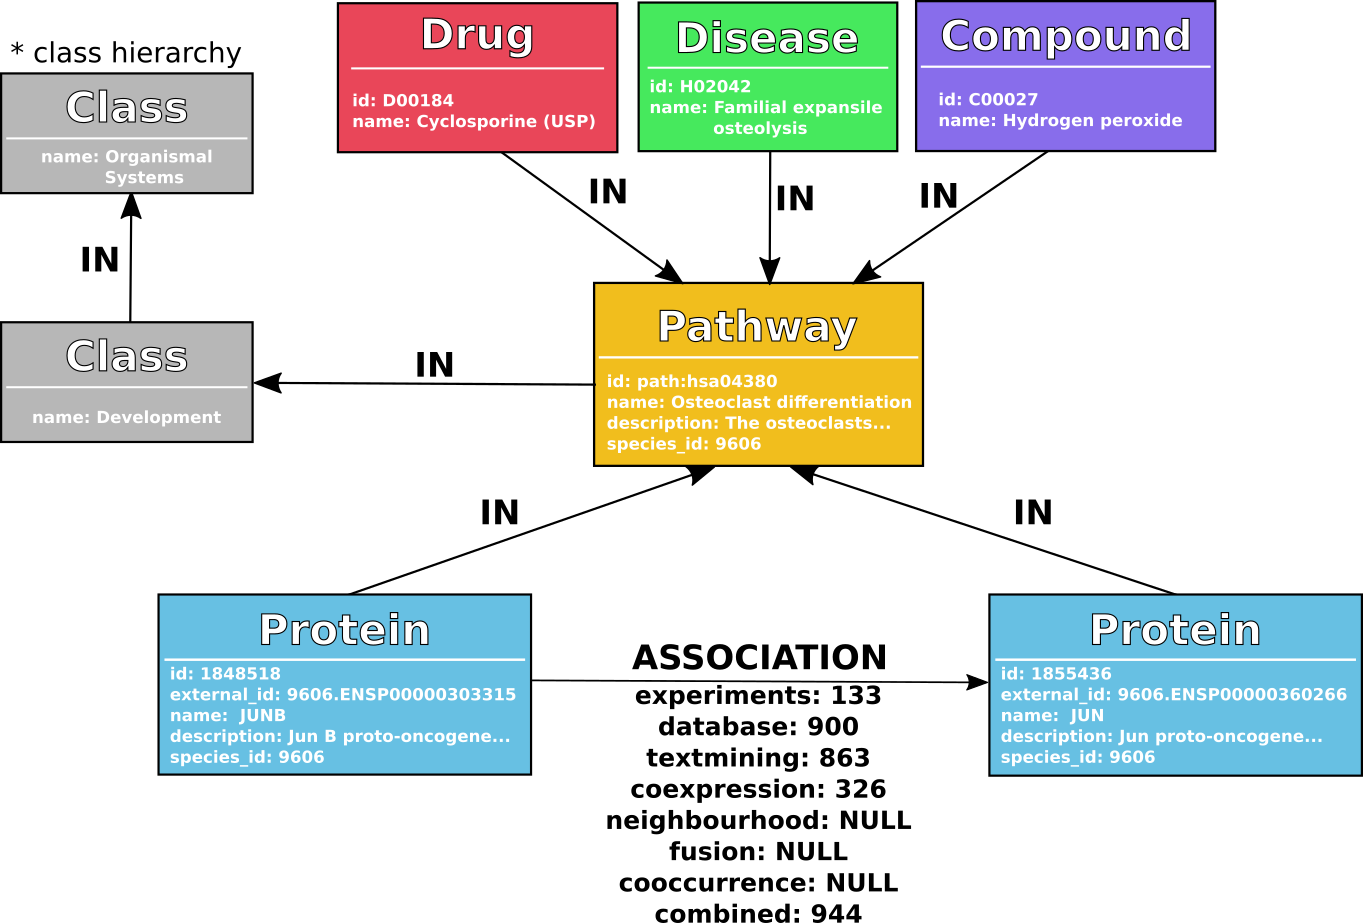
\includegraphics[width=0.9\linewidth]{database_scheme.png}
    % NOTE: neighbourhood, fusion and cooccurence are available only for bacteria and archea
\end{figure}
\end{frame}

\begin{frame}{Workflow}
% NOTE:
% q-gram indexing is used to do the fuzzy search and map query strings to protein IDs
% More: https://www.YouTube.com/watch?v=I39Rhegg8Xg

% NOTE:
% Vue.js is a MVC framework, vis.js was used to draw the network
% and jQuery was used to handle UI

% NOTE:
% Why Docker? Makes deployment really easy

\begin{figure}
    \centering
    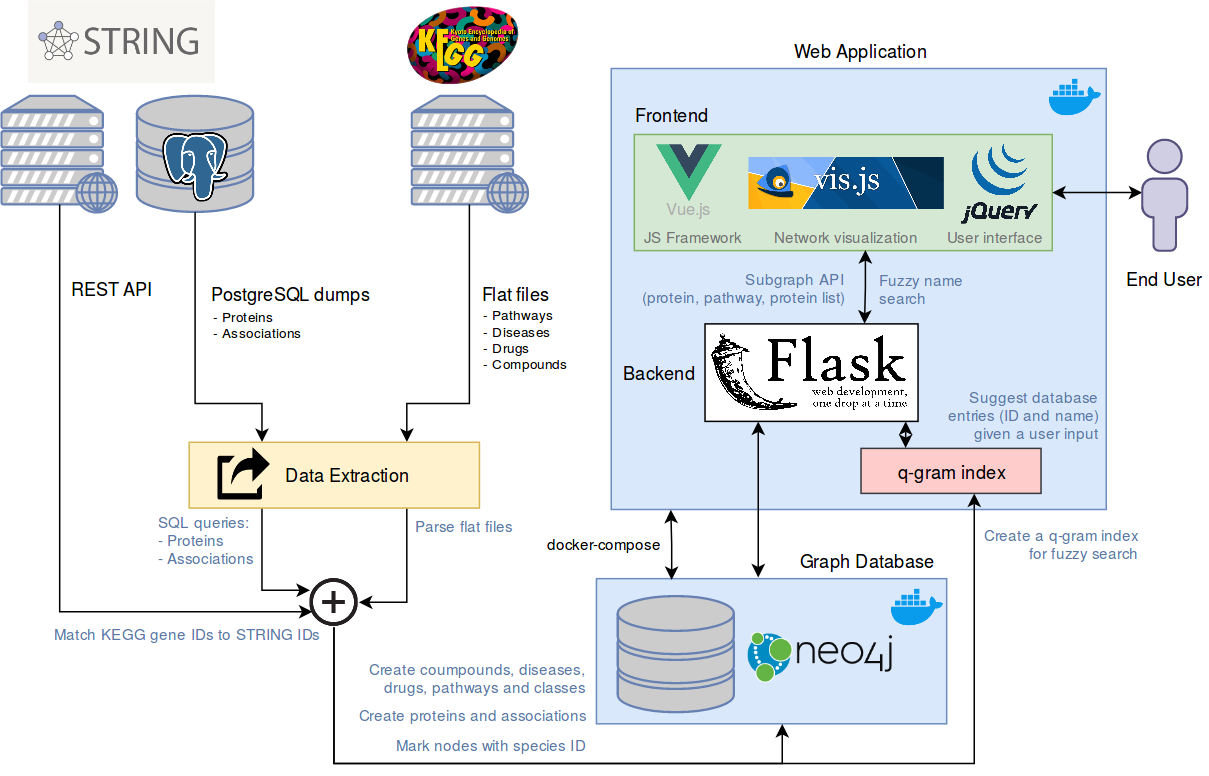
\includegraphics[width=\linewidth]{workflow.png}
\end{figure}
\end{frame}

\section{Results}

\definecolor{protein}{HTML}{178ab7}
\definecolor{disease}{HTML}{15a52f}
\definecolor{compound}{HTML}{8f17b7}

\begin{frame}{Protein Graph DB in numbers}
% NOTE:
% Disease, Drug and Compound are only available for human
% MATCH ()-[a:ASSOCIATION]->()
% WHERE a.combined >= 700
% RETURN COUNT(a)
% Put threshold-#edges plot
\begin{itemize}
    \item Species: Homo sapiens (human) \& Mus musculus (house mouse)
    \vfill
    \item Nodes
    \begin{itemize}
        \item \textcolor{protein}{Protein}: 43 125
        \item \textcolor{orange}{Pathway}: 646
        \item \textcolor{red}{Drug}: 3 731
        \item \textcolor{disease}{Disease}: 969
        \item \textcolor{compound}{Compound}: 3 465
        \item \textcolor{gray}{Class}: 49
    \end{itemize}
    \vfill
    \item Relationships
        \begin{itemize}
        \item \textbf{ASSOCIATION}: 11 983 549
        \item \textbf{IN}: 76 715
    \end{itemize} 
\end{itemize}
\end{frame}

\begin{frame}{Protein Graph DB in numbers}
    \begin{figure}
        \centering
        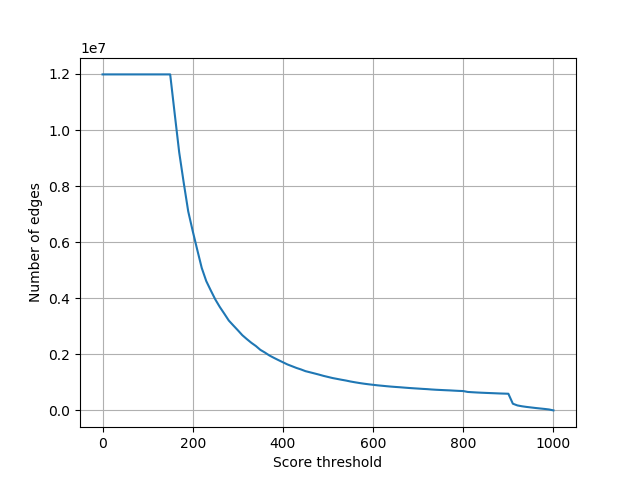
\includegraphics[width=0.8\linewidth]{threshold_vs_edges.png}
    \end{figure}
\end{frame}

%------------------------------------------------

\begin{frame}{Protein subgraph (example)}
% NOTE:
% Scores are in range [0, 1000]
% <id> is the internal ID that Neo4j assigns to each node and relationship
% In our case, the direction of relationship is not important
\begin{figure}
    \centering
    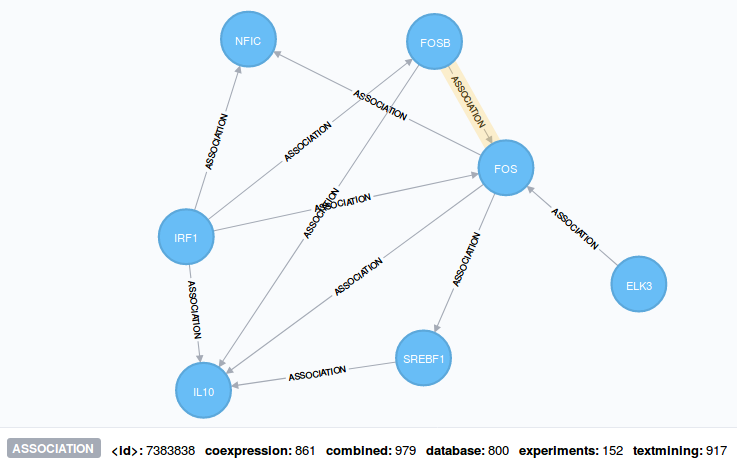
\includegraphics[width=0.8\linewidth]{protein_graph.png}
\end{figure}
\begin{figure}
    \centering
    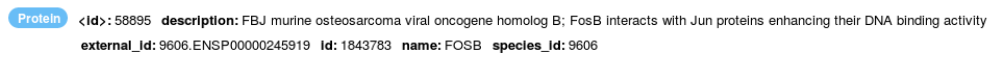
\includegraphics[width=0.9\linewidth]{protein_attributes.png}
\end{figure}
\end{frame}

\begin{frame}{Query: Central proteins}
$  T_i = |\{j : j \in \mathcal{N}(i), s_{ij} \geqslant \text{threshold}\}| $
\begin{block}{Cypher}
% NOTE:
% In reality, our queries use protein IDs (from fuzzy search) instead of protein names.
% That way we avoid ambiguities.
% 9606 is the ID of human
% \scriptsize
% WITH ["SFPI1", "FOSB", "MLXIPL", ...] AS protein\_names, \newline
% 9606 AS species\_id, \newline
% 700 AS threshold \newline
% MATCH (p1:Protein \{species\_id: species\_id\})-[a:ASSOCIATION]-(p2:Protein \{species\_id: species\_id\}) \newline
% WHERE p1.name IN protein\_names AND p2.name IN protein\_names AND ID(p1) <> ID(p2) AND a.combined >= threshold \newline
% RETURN p1.name AS name, SUM(SIZE((p1)-[a]-(p2))) AS degree \newline
% ORDER BY degree DESC
\begin{figure}
    \centering
    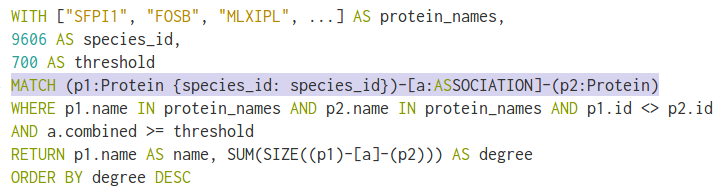
\includegraphics[width=\linewidth]{central_proteins_query.png}
\end{figure}
\end{block}
\vfill
\begin{block}{Output}
\scriptsize
    \begin{tabular}{| l | l |}
        \hline
        name & degree \\ \hline \hline
        JUN & 25 \\ \hline
        FOS & 19 \\ \hline
        CREB1 & 14 \\ \hline
        ... & ... \\
        \hline
    \end{tabular}
\end{block}
\end{frame}


\begin{frame}{Query: Common pathways}
- Common pathways given a protein list
\begin{block}{Cypher}
% \scriptsize
% WITH ["SFPI1", "FOSB", "MLXIPL", ...] AS protein\_names, \newline
% 9606 AS species\_id \newline
% MATCH (protein:Protein \{species\_id: species\_id\})-[element:IN]->(pathway:Pathway) \newline
% WHERE protein.name IN protein\_names \newline
% RETURN DISTINCT pathway.name AS pathway, COUNT(element) AS n\_proteins \newline
% ORDER BY n\_proteins DESC
\begin{figure}
    \centering
    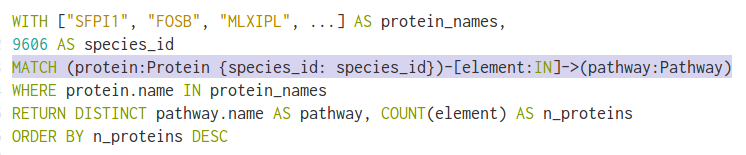
\includegraphics[width=\linewidth]{common_pathways_query.png}
\end{figure}
\end{block}
\vfill
\begin{block}{Output}
\small
\begin{tabular}{|l|l|}
    \hline
    pathway & n\_proteins\\ \hline \hline
    Transcriptional misregulation in cancer & 14\\ \hline
    Human T-cell leukemia virus 1 infection & 12\\ \hline
    Pathways in cancer & 12\\ \hline
    ... & ...\\
    \hline
\end{tabular}
\end{block}
\end{frame}


\begin{frame}{Query: Common diseases}
- Common diseases implicated by associated pathways given a protein list
\begin{block}{Cypher}
% \scriptsize
% WITH ["SFPI1", "FOSB", "MLXIPL", ...] AS protein\_names, \newline
% 9606 AS species\_id \newline
% MATCH (protein:Protein \{species\_id: species\_id\})-[:IN]->(pathway:Pathway)<-[:IN]-(disease:Disease) \newline
% WHERE protein.name IN protein\_names \newline
% WITH disease, pathway, COUNT(protein) AS n\_proteins \newline
% RETURN disease.name AS disease, COUNT(pathway) AS n\_pathways, n\_proteins \newline
% ORDER BY n\_proteins DESC
\begin{figure}
    \centering
    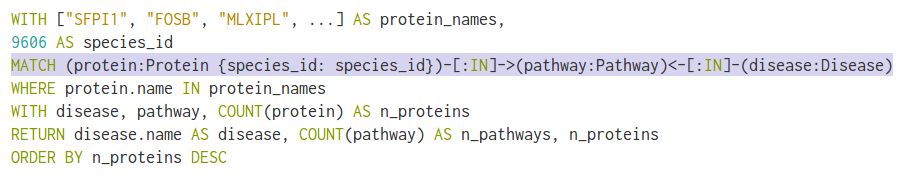
\includegraphics[width=\linewidth]{common_diseases_query.png}
\end{figure}
\end{block}
\vfill
\begin{block}{Output}
\small
\begin{tabular}{|l|l|l|}
    \hline
    disease & n\_pathways & n\_proteins\\ \hline \hline
    Pituitary adenomas & 1 & 14 \\ \hline
    Hairy-cell leukemia & 1 & 14 \\ \hline
    Acute myeloid leukemia (AML) & 1 & 14 \\ \hline
    ... & ... & ...\\
    \hline
\end{tabular}
\end{block}
\end{frame}


\begin{frame}{Query: Module detection}
\begin{block}{Cypher}
% NOTE:
% Graph algorithms library doesn't come with default Neo4j installation.
% A .jar file needs to be downloaded and whitelisted in the Neo4j configuration file
% https://github.com/neo4j-contrib/neo4j-graph-algorithms/releases
% \small
% CALL algo.louvain.stream('Protein', 'ASSOCIATION', \{\}) \newline
% YIELD nodeId, community \newline
% RETURN COLLECT(nodeId) AS protein\_ids, community \newline
% ORDER BY community
% NOTE:
% Instead of returning node ID and community ID pair in each row,
% COLLECT is used to join all node IDs into one row
\begin{figure}
    \centering
    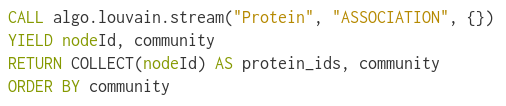
\includegraphics[width=\linewidth]{module_detection_query.png}
\end{figure}
\end{block}
\vfill
\begin{block}{Output}
\small
\begin{tabular}{|l|l|}
    \hline
    protein\_ids & community \\ \hline \hline
    [29451,29452,29453,...] & 0 \\ \hline
    [29815,29899,30082,...] & 1 \\ \hline
    [29858] & 2 \\ \hline
    ... & ... \\
    \hline
\end{tabular}
\end{block}
\end{frame}


\begin{frame}
\centering
\href{http://localhost:5000/}{\huge{Web server (live demo)}}
\end{frame}



\section{Next steps}
\begin{frame}{Next steps}
\begin{itemize}
    \item Extend the database
    \begin{itemize}
        \item Protein - protein actions
        % NOTE:
        % We only have ID and name for drugs, diseases and compounds
        % Those other KEGG databases contain other info (such as description)
        \item \href{https://www.genome.jp/kegg/drug/}{KEGG DRUG}
        \item \href{https://www.genome.jp/kegg/disease/}{KEGG DISEASE}
        \item \href{https://www.genome.jp/kegg/compound/}{KEGG COMPOUND}
    \end{itemize}
    \vfill
    \item Include other species
    \vfill
    \item Production-level web server
    \vfill
    \item Explore the possibility of a graph-native machine learning system
\end{itemize}
\end{frame}

\begin{frame}
\centering
\huge{Thank you :)}
\bigskip \\
\small{
    \href{https://backofenlab.github.io/protein-graph-database/}{https://backofenlab.github.io/protein-graph-database/} \\
    \href{https://github.com/BackofenLab/protein-graph-database}{https://github.com/BackofenLab/protein-graph-database}
}

\begin{columns}
\begin{column}{0.6\textwidth}
   \begin{figure}
    \centering
    
\includegraphics[width=0.6\linewidth]{neuromac.jpeg}
    \end{figure}
\end{column}
\begin{column}{0.4\textwidth}  %%<--- here
\begin{figure}
    \centering
    
\includegraphics[width=0.5\linewidth]{bioinf-fr-logo-blau.jpg}
\end{figure}
\end{column}
\end{columns}
\vfill
\begin{itemize}
    \item Special thanks to Prof. Rolf Backofen and Stefan Jankowski 
\end{itemize}
\end{frame}

\end{document}